
\documentclass[12pt]{article}

\usepackage[utf8]{inputenc}
\usepackage[greek, english]{babel}
\usepackage{caption, graphicx, alphabeta, amsfonts, amsmath, amssymb, amsthm, latexsym, MnSymbol, stackrel, titlesec}

\newcommand{\R}{\mathbb{R}}
\newcommand{\N}{\mathbb{N}}
\newcommand{\norm}[1]{\left\lVert#1\right\rVert}
\newcommand{\margin}{\hspace{4pt}}
\newcommand{\centered}[1]{\begin{align*}#1\end{align*}}

\newenvironment{rcases}
	{\left.\begin{aligned}}
	{\end{aligned}\right\rbrace}

\setlength{\parindent}{0in}
\setlength{\oddsidemargin}{0in}
\setlength{\textwidth}{6.5in}
\setlength{\textheight}{10in}
\setlength{\topmargin}{-1.0in}
\setlength{\headheight}{18pt}

\titlespacing*{\subsection}
{0pt}{5.5ex plus 1ex minus .2ex}{4.3ex plus .2ex}

\title{\hugeΑλγοριθμική Επιχειρησιακή Έρευνα\\Δεύτερη Εργασία}
\author{Σιώρος Βασίλειος\\Ανδρινοπούλου Χριστίνα}
\date{Οκτώβριος 2019}

\begin{document}

\maketitle

\thispagestyle{empty}

\pagenumbering{arabic}



\pagebreak

\subsection*{1. Find a differentiable function f : R R such that f does not have an extremum at its
critical point.}

\begin{figure}[hp]
    \centering
    \captionsetup{justification=centering}

    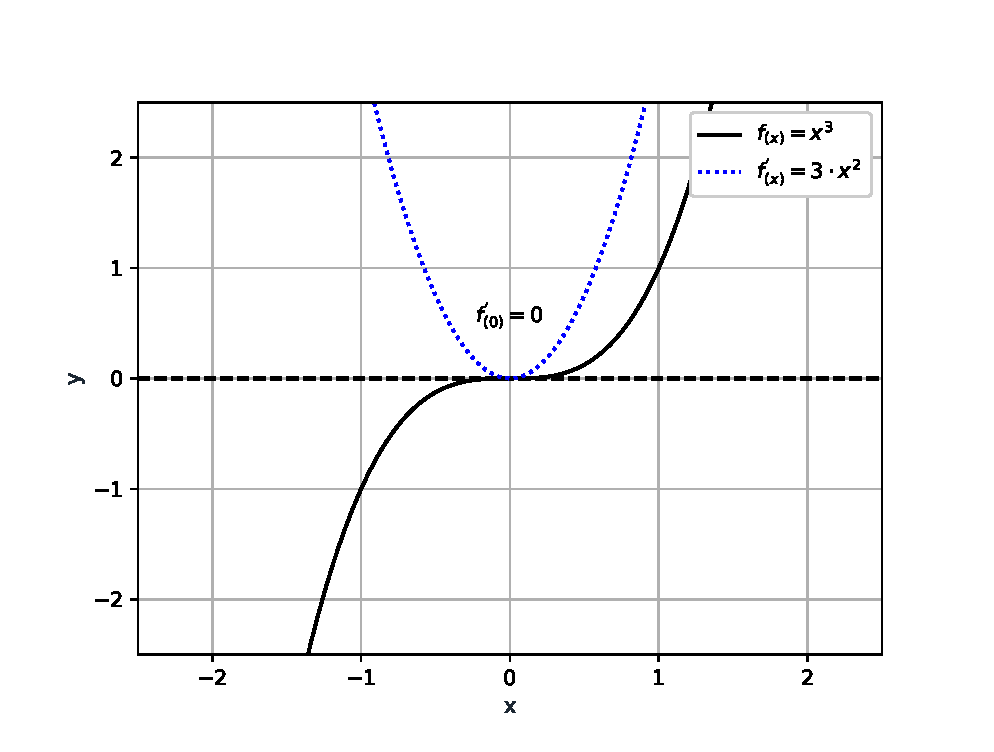
\includegraphics{cubic_figure}
    \caption{An example of a differentiable function \( f: \R \rightarrow \R \) which does not have an extremum at its critical point}
\end{figure}

\vspace{2in}


\pagebreak

\subsection*{2. Given a positive integer S, which decompositions
a1 + + an = S
with the ai positive integers have the largest product a1 an?}

\vspace{2in}


\pagebreak

\subsection*{3. Find the optimal solution to the Diet Problem when the cost function is
Cost(x1, x2) = x1 + x2.}

\begin{figure}[hp]
    \centering
    \captionsetup{justification=centering}

    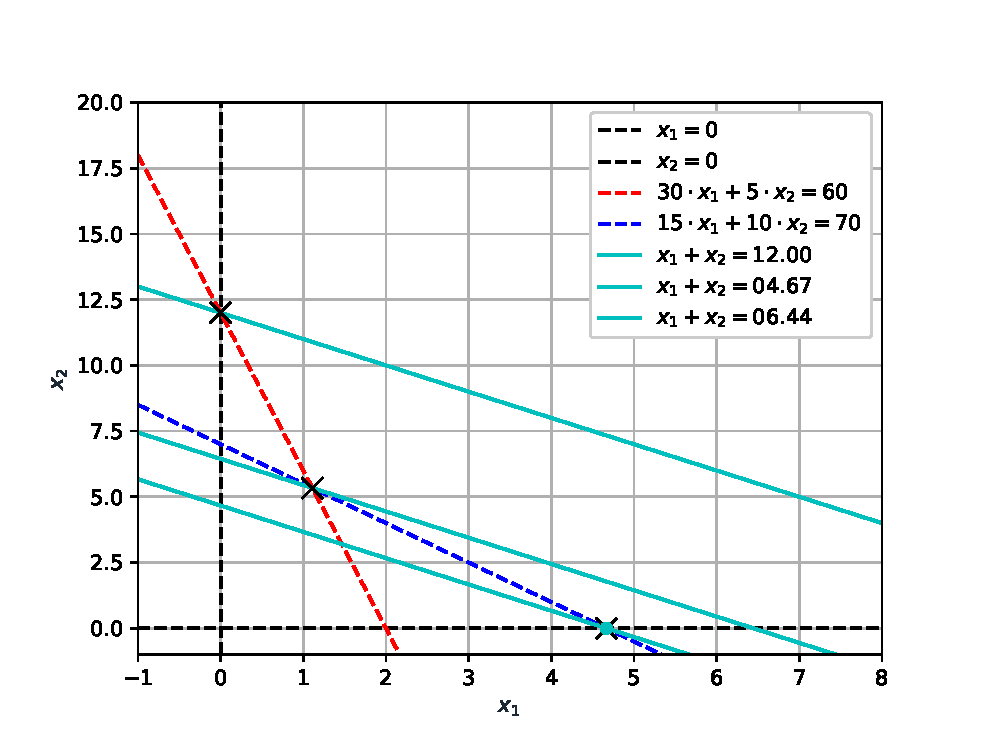
\includegraphics{diet_problem_figure}
    \caption{The Optimal Solution to the Diet Problem when the total cost is given by the function $Cost(x_1, x_2) = x_1 \cdot x_2$}
\end{figure}

\vspace{2in}


\pagebreak

\subsection*{4. Let A,B Rnn. Show that the traditional way of computing their product AB requires
a total of (2n 1)n2 arithmetic operations.}

\vspace{2in}


\pagebreak

\subsection*{5. Consider the problem of solving a system of n linear equations in n unknowns. Show
that the Gaussian elimination method requires O(n3) arithmetic operations in order to either
compute a solution or to decide that no solution exist.}

\vspace{2in}


\pagebreak

\subsection*{6. Suppose that we are given a set of vectors in Rn that form a basis and let y be an
arbitrary vector in Rn. We wish to express y as a linear combination of the basis vectors. How
can this by accomplished?}

\vspace{2in}


\pagebreak

\subsection*{7. Study the paper with title: Do dogs know Calculus? found in the Readings folder.}

\vspace{2in}

\end{document}
